\documentclass{ifacconf}

\usepackage{natbib}            % you should have natbib.sty
\usepackage[utf8]{inputenc}    % Eingabe von Umlauten im Editor, dieser sollte dann auch auf utf8 Encoding eingestellt sein
\usepackage{graphicx}          % Include this line if your 
                               % document contains figures,
%\usepackage[dvips]{epsfig}    % or this line, depending on which
                               % you prefer.
                               
\usepackage{units}
\usepackage{hyperref}

% for German
% \usepackage{ngerman}           % neue Deutsche Rechtschreibung, Silbentrennung
% \usepackage[T1]{fontenc}       % Trennung mit Umlauten

% to include tikz pictures of figure created with matlab2tikz, see also file ``plotFigureTest.m''
\usepackage{tikz}
\usepackage{pgfplots}
\pgfplotsset{compat=newest}  % use newest version of pgfplots
\usepackage{amsmath}  % useful for math

% to include the legend into the caption. The commands are
%\mlLineLegend{red}
%\mlLineLegendDashed{red}
%\mlLineLegendDotted{red}
%\mlLineLegendDashDotted{red}
%\mlPointLegend{red}
\newlength{\mlLegendThickness}
\setlength{\mlLegendThickness}{0.4mm}
\newlength{\mlLegendHeight}
\setlength{\mlLegendHeight}{0.6ex}
\newcommand{\mlLineLegend}[1]{\mbox{\color{#1}
\protect\rule[\mlLegendHeight]{3mm}{\mlLegendThickness}\hspace*{-1mm}
}}
\newcommand{\mlLineLegendDashed}[1]{\mbox{\color{#1}
\protect\rule[\mlLegendHeight]{1.5mm}{\mlLegendThickness}\hspace*{0mm}
\protect\rule[\mlLegendHeight]{1.5mm}{\mlLegendThickness}\hspace*{-1mm}
}}
\newcommand{\mlLineLegendDotted}[1]{\mbox{\color{#1}
\protect\rule[\mlLegendHeight]{0.4mm}{\mlLegendThickness}\hspace*{0mm}
\protect\rule[\mlLegendHeight]{0.4mm}{\mlLegendThickness}\hspace*{0mm}
\protect\rule[\mlLegendHeight]{0.4mm}{\mlLegendThickness}\hspace*{0mm}
\protect\rule[\mlLegendHeight]{0.4mm}{\mlLegendThickness}\hspace*{-1mm}
}}
\newcommand{\mlLineLegendDashDotted}[1]{\mbox{\color{#1}
\protect\rule[\mlLegendHeight]{1.5mm}{\mlLegendThickness}\hspace*{0mm}
\protect\rule[\mlLegendHeight]{0.4mm}{\mlLegendThickness}\hspace*{0mm}
\protect\rule[\mlLegendHeight]{1.5mm}{\mlLegendThickness}\hspace*{0mm}
\protect\rule[\mlLegendHeight]{0.4mm}{\mlLegendThickness}\hspace*{-1mm}
}}
\newcommand{\mlPointLegend}[1]{\mbox{\color{#1}
\protect\rule[\mlLegendHeight]{0.4mm}{\mlLegendThickness}\hspace*{-0.75mm}
}}

\begin{document}

\begin{frontmatter}

\title{Laborprotocol BMo2-1}


% include all authors, underline corresponding author
\author{E. Boateng,} 
\author{J. Qin} 
% \author{}

\begin{abstract}                          % Abstract of not more than 250 words.
This protocol for L1 and H1 is concerned with the experimental setup. A qualified model of the dynamics were derived and missing parameters of the model were identified.
\end{abstract}

\end{frontmatter}

\section{Work tasks}
First, to be familiar with the experimental setup. A strategy should be develpoed to solve the main task of the lab course. In addition, a system need to be modeled with an adequate precision and linearized.


\section{Simulation model of the helicopter}

In order to be able to design controllers during L2, the helicopter system has to be modeled. Because the complete model of the helicopter is very complicated, simplification of the model while keeping the model complexity within an acceptable range is necessary.

Figure 1 shows the simplified model with the corresponding
parameters.

Applying the law of angular momentum to the axes a,b and c, the following equations are derived.


\begin{align}	
&\Theta_a\ddot{\alpha} = -\cos(\beta)L_2\sin(\gamma)(F_f+F_b)\\
&\Theta_b\ddot{\beta} = \cos(\gamma)L_2(F_f+F_b)-\cos(\beta)(mL_1-ML_2)g\\
&\Theta_c\ddot{\gamma} = \frac{L_3}{2}(F_f-F_b)
\end{align}

$\Theta_a$, $\Theta_b$ and $\Theta_c$ are the moment of inertia with respect to the axes a,b and c. Their values can be calculated by the following equations.

\begin{align}
\Theta_a &= mL_1^2 + ML_2^2\\
\Theta_b &= mL_1^2 + ML_2^2\\
\Theta_c &= \frac{1}{6}m(\frac{L3}{2})^2
\end{align}


\begin{figure} % use \begin{figure*} for two-column figure
\begin{center} 
% the variable for the width of the figure which you created with matlab2tikz has to be defined and set
\newlength{\figurewidth} % ... defined
\setlength{\figurewidth}{0.8\columnwidth} % ...set 
% for details see file ``plotFigureTest.m''
%% This file was created by matlab2tikz.
%
%The latest updates can be retrieved from
%  http://www.mathworks.com/matlabcentral/fileexchange/22022-matlab2tikz-matlab2tikz
%where you can also make suggestions and rate matlab2tikz.
%
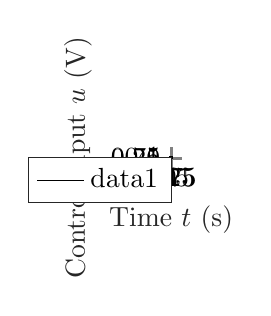
\begin{tikzpicture}

\begin{axis}[%
width=0.951\figurewidth,
height=0.75\figurewidth,
at={(0\figurewidth,0\figurewidth)},
scale only axis,
xmin=0,
xmax=1,
xtick={   0, 0.25,  0.5, 0.75,    1},
xlabel style={font=\color{white!15!black}},
xlabel={Time $t$ (s)},
ymin=0,
ymax=1,
ytick={   0, 0.25,  0.5, 0.75,    1},
ylabel style={font=\color{white!15!black}},
ylabel={Control input $u$ (V)},
axis background/.style={fill=white},
xmajorgrids,
ymajorgrids,
legend style={legend cell align=left, align=left, draw=white!15!black}
]
\addplot [color=black]
  table[row sep=crcr]{%
0	0\\
0.01	0.00999983333416666\\
0.02	0.0199986666933331\\
0.03	0.0299955002024957\\
0.04	0.0399893341866342\\
0.05	0.0499791692706783\\
0.06	0.0599640064794446\\
0.07	0.0699428473375328\\
0.08	0.0799146939691727\\
0.09	0.089878549198011\\
0.1	0.0998334166468282\\
0.11	0.109778300837175\\
0.12	0.119712207288919\\
0.13	0.129634142619695\\
0.14	0.139543114644236\\
0.15	0.149438132473599\\
0.16	0.159318206614246\\
0.17	0.169182349066996\\
0.18	0.179029573425824\\
0.19	0.188858894976501\\
0.2	0.198669330795061\\
0.21	0.2084598998461\\
0.22	0.218229623080869\\
0.23	0.227977523535188\\
0.24	0.237702626427135\\
0.25	0.247403959254523\\
0.26	0.257080551892155\\
0.27	0.266731436688831\\
0.28	0.276355648564114\\
0.29	0.285952225104836\\
0.3	0.29552020666134\\
0.31	0.305058636443443\\
0.32	0.314566560616118\\
0.33	0.324043028394868\\
0.34	0.333487092140814\\
0.35	0.342897807455451\\
0.36	0.35227423327509\\
0.37	0.361615431964962\\
0.38	0.370920469412983\\
0.39	0.380188415123161\\
0.4	0.389418342308651\\
0.41	0.398609327984423\\
0.42	0.40776045305957\\
0.43	0.416870802429211\\
0.44	0.425939465066\\
0.45	0.43496553411123\\
0.46	0.44394810696552\\
0.47	0.452886285379068\\
0.48	0.461779175541483\\
0.49	0.470625888171158\\
0.5	0.479425538604203\\
0.51	0.488177246882908\\
0.52	0.496880137843737\\
0.53	0.505533341204847\\
0.54	0.514135991653113\\
0.55	0.522687228930659\\
0.56	0.531186197920883\\
0.57	0.539632048733969\\
0.58	0.548023936791874\\
0.59	0.556361022912784\\
0.6	0.564642473395035\\
0.61	0.572867460100481\\
0.62	0.581035160537305\\
0.63	0.58914475794227\\
0.64	0.597195441362392\\
0.65	0.605186405736039\\
0.66	0.613116851973434\\
0.67	0.62098598703656\\
0.68	0.628793024018468\\
0.69	0.636537182221968\\
0.7	0.644217687237691\\
0.71	0.651833771021537\\
0.72	0.659384671971473\\
0.73	0.666869635003698\\
0.74	0.674287911628145\\
0.75	0.681638760023334\\
0.76	0.688921445110551\\
0.77	0.696135238627357\\
0.78	0.70327941920041\\
0.79	0.710353272417608\\
0.8	0.717356090899523\\
0.81	0.724287174370143\\
0.82	0.731145829726896\\
0.83	0.737931371109963\\
0.84	0.744643119970859\\
0.85	0.751280405140293\\
0.86	0.757842562895277\\
0.87	0.764328937025505\\
0.88	0.770738878898969\\
0.89	0.777071747526824\\
0.9	0.783326909627483\\
0.91	0.78950373968995\\
0.92	0.795601620036366\\
0.93	0.801619940883777\\
0.94	0.807558100405114\\
0.95	0.813415504789374\\
0.96	0.819191568300998\\
0.97	0.82488571333845\\
0.98	0.83049737049197\\
0.99	0.836025978600521\\
1	0.841470984807897\\
};
\addlegendentry{data1}

\end{axis}
\end{tikzpicture}% % inclusion of tikz-code
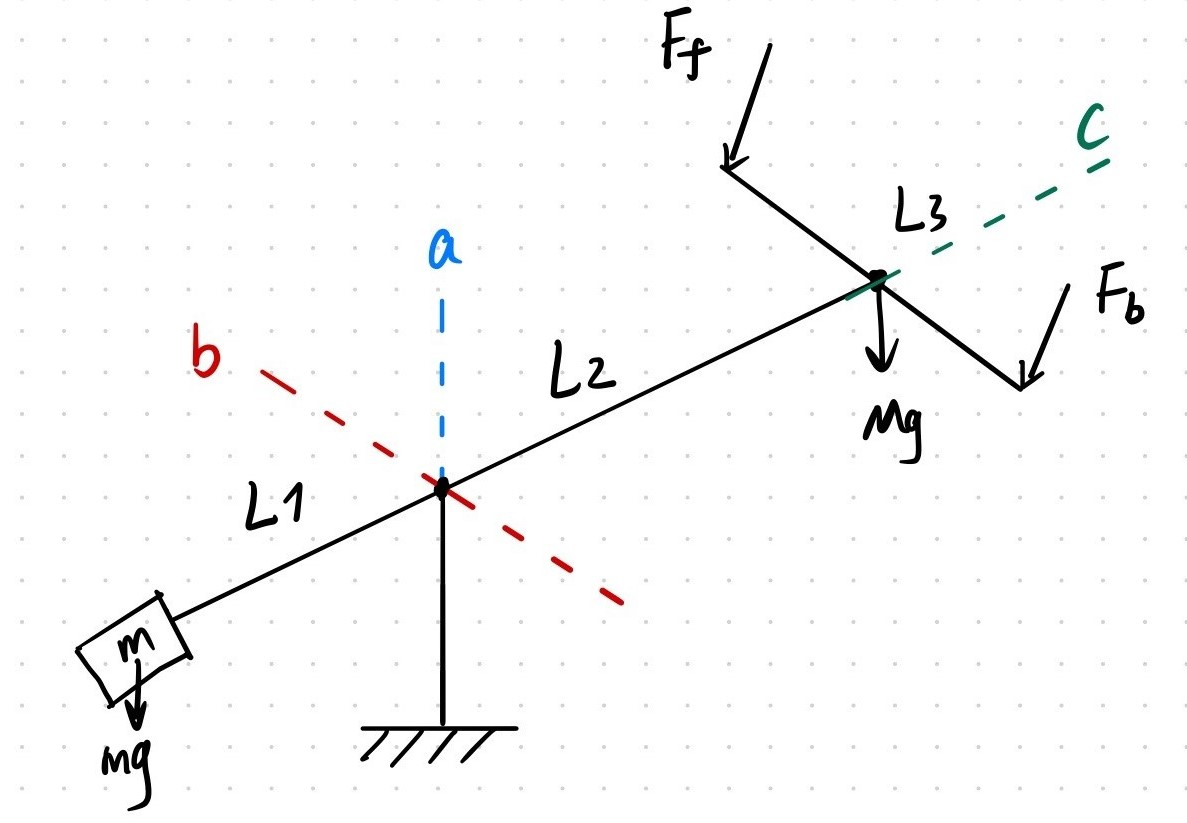
\includegraphics[width=\columnwidth]{model} % inclusion of pdf
\caption{simplified model of the helicopter}
\label{model}
		
\end{center}
\end{figure}


The state vector $x =\begin{bmatrix}
	\alpha&\beta&\gamma&\dot{\alpha}&\dot{\beta}&\dot{\gamma}
\end{bmatrix}^T$ and the input vector $u = \begin{bmatrix}
F_f&F_b
\end{bmatrix}^T$. Therefore, $\dot{x} = \begin{bmatrix}
\dot{\alpha}&\dot{\beta}&\dot{\gamma}&\ddot{\alpha}&\ddot{\beta}&\ddot{\gamma}
\end{bmatrix}^T$ can be displayed as follows.
\begin{equation}
\dot{x}=\begin{bmatrix}
	\dot{\alpha}\\
	\dot{\beta}\\
	\dot{\gamma}\\
	\frac{-\cos(\beta)L_2\sin(\gamma)(F_f+F_b)}{mL_1^2 + ML_2^2}\\
	\frac{\cos(\gamma)L_2(F_f+F_b)-\cos(\beta)(mL_1-ML_2)g}{mL_1^2 + ML_2^2}\\
	\frac{\frac{L_3}{2}(F_f-F_b)}{\frac{1}{6}m(\frac{L3}{2})^2}
\end{bmatrix}
\end{equation}

\section{Voltage Model}

Data of the dependency between the voltage and the corresponding forces of the propeller were provided. Analysis of the data shows a quadratic curve relationship between the Forces and the applied voltage. Using curve fitting methods (\mathit{polyfit} Matlab command), the exact parameters of the curve are obtained to be able to model the force dependency for any given decimal voltage. 
The derived coefficients and the corresponding equation the force as a function of the voltage is:
\begin{align}
 F_f  (V) = 6.156*V^2 +	-0.1342*V 	-0.13917 \\
 F_b (V) = 4.704*V^2 +	0.00510*V 	-0.278
 \end{align}
 
 A plot of the forces over a voltage spectrum is illustrates in Figure 2.
 
\begin{figure}
\begin{center}
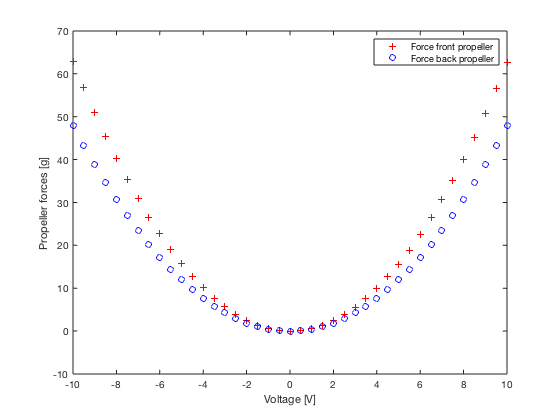
\includegraphics[width=\columnwidth]{Voltage_Forces.png}
\caption{Plot of propeller forces over voltage}
\label{Figure 2}
\end{center}
\end{figure}

%The protocols have to be typeset with \LaTeX. A good German introduction to \LaTeX can be found in \citep{hagenEinfuehrung}. An alternative in English is \citep{lshort}. A short guide concerning the mathematical part is given by \citep{mathGuide}.

\section{Plant model}

Using the equation of the simplified physical model of the helicopter discussed in \hyperref[Simulation model of the helicopter]{section 2}, the mathematical state space model of the plant is derived by linearization of $\dot{x}$ w. r. t. ${x} $ to derive the A matrix and $\dot{x}$  w. r. t.  $u$ to derive the B matrix.

The resulting computation in Matlab yields:


$A = \begin{bmatrix}
0 & 0 & 0 & 1 & 0 & 0\\
0 & 0 & 0 & 0 & 1 & 0\\
0 & 0 & 0 & 0 & 0 & 1\\
0 & \frac{(\sin(\beta)\sin(\gamma)L_2(F_b + F_f)}{mL_1^2 + ML_2^2} & -\frac{\cos(\beta)\cos(\gamma)L2(F_b + (F_f)}{mL_1^2 + M*L_2^2)} & 0 & 0 & 0\\
0 & -\sin(\beta)gL_2M - L_1m & -\frac{\sin(\gamma)L_2(F_b + F_f)}{mL_1^2 + ML_2^2} & 0 & 0 & 0\\
0 & 0 & 0 & 0 & 0 & 0
\end{bmatrix}$

$B = \begin{bmatrix}
0 & 0\\
0 & 0\\
0 & 0\\
-\frac{\cos(\beta)\sin(\gamma)L_2}{mL_1^2 + ML_2^2} & \frac{\cos(\beta)\sin(\gamma)L2}{mL_1^2 + ML_2^2}\\
\frac{\cos(\gamma)L_2}{mL_1^2 + ML_2^2} & \frac{\cos(\gamma)L_2}{mL_1^2 + ML_2^2}\\
\frac{12}{mL_3} & -\frac{12}{mL_3}\\
\end{bmatrix}$
 
 

For the next Lab session, the following draft working plan detailed in Table~\ref{table:working plan}  will be used  Table~\ref{table:working plan}.

\section{Comments}

Since the physical model of the helicopter has been simplified, our validation of the model demonstrated deviations from the provided blackbox model. These simplifications will be considered in the design of the controller.  



\begin{table*}
\caption{Working Plan for L2.}
\label{table:working plan}
\centering
\begin{tabular}{|c|c|p{4.5cm}|p{4.5cm}|p{4.5cm}|}
\hline
\bfseries Time & \bfseries Duration & \bfseries Goal & \bfseries Task & \bfseries Preparation\\ \hline \hline
14:00 & 30 min. & Test File to actuate motor & Create Quarc Simulink File & Read Quarc documentation \\ \hline
 14:30 & 1,5 hour  & Design a controller  & Choose a suitable controller  &  Review KRT lecture notes\\ \hline
 15:30 & 1,5 hour &  Trajectory planning & Develop optimal trajectory for helicopet tasl & Review KRT lecture videos and script \\ \hline
 &  &  &  &  \\ \hline
 &  &  &  &  \\ \hline
\end{tabular}
\end{table*}




%\bibliographystyle{alpha}        % Include this if you use bibtex 
%\bibliography{autosam}           % and a bib file to produce the 
%\bibliography{autosam}
                                 % bibliography (preferred). The
                                 % correct style is generated by
                                 % Elsevier at the time of printing.
                                 

\begin{thebibliography}{3}


\bibitem[Quanser Inc.(2010)]{hagenEinfuehrung}
Quanser Inc. (2011).
\newblock 3-DOF Helicopter: User Manual'.
\newblock


\bibitem[Control of a 3-DOF Helicopter]{Handbook}
Control of a 3-DOF Helicopter.
\newblock Handbook for Laboratory Course "Concepts of Automatic Control".
\newblock Corona Edition, Winter term 2020/21.
\end{thebibliography}

%\appendix
\end{document}
